\documentclass[aspectratio=169,11pt]{beamer}
% Shared house style for the AI Trading 24/7 modular documents.
% Every module \input's this file, then sets its own \title block and body.
% Derived from the former InfrastructureSetup.tex / ReplicationExecutionFlow.tex preambles.

% Beamer supplies its own page layout, headings, lists, and page furniture.
\newif\ifaitradingbeamer
\makeatletter
\@ifclassloaded{beamer}{\aitradingbeamertrue}{\aitradingbeamerfalse}
\makeatother
\ifaitradingbeamer\else
\usepackage[top=1in, bottom=1in, left=1.1in, right=1.1in]{geometry}
\fi
\usepackage{microtype}
\usepackage{libertine}
\usepackage[libertine]{newtxmath}
\usepackage[T1]{fontenc}
\usepackage{amsmath}
\ifaitradingbeamer\else
\usepackage{enumitem}
\usepackage{setspace}
\usepackage{titlesec}
\fi
\usepackage{xcolor}
\ifaitradingbeamer\else
\usepackage{fancyhdr}
\fi
\usepackage{longtable}
\usepackage{booktabs}
\usepackage{array}
\usepackage{tabularx}
\usepackage{seqsplit}
\usepackage{hyperref}
\usepackage{xurl}

% Colors
\definecolor{uablue}{RGB}{0,56,107}
\definecolor{sectiongray}{RGB}{64,64,64}
\definecolor{accent}{RGB}{150,0,24}
\definecolor{definitiongreen}{RGB}{0,102,51}

% Header (each module may override \fancyhead[L] after \input if it wishes)
\ifaitradingbeamer\else
\pagestyle{fancy}
\fancyhf{}
\fancyhead[L]{\small\textcolor{uablue}{AI Trading 24/7: Step-by-Step Build}}
\fancyhead[R]{\small\textcolor{uablue}{Muting (Don) Ma}}
\fancyfoot[C]{\thepage}
\renewcommand{\headrulewidth}{0.5pt}

% Section format
\titleformat{\section}
  {\color{uablue}\normalfont\large\bfseries}
  {\thesection.}{0.5em}{}[\color{uablue}\titlerule]
\titleformat{\subsection}
  {\color{sectiongray}\normalfont\normalsize\bfseries}
  {\thesubsection}{0.5em}{}
\titlespacing*{\section}{0pt}{1.4ex plus 0.5ex minus .2ex}{0.8ex plus .2ex}
\titlespacing*{\subsection}{0pt}{1.0ex plus 0.4ex minus .2ex}{0.5ex plus .2ex}
\newcommand{\sectionbreak}{\clearpage}

\setstretch{1.08}
\setlength{\parskip}{0.45em}
\setlength{\parindent}{0pt}
\fi
\setlength{\emergencystretch}{3em}
\hypersetup{colorlinks=true, linkcolor=uablue, urlcolor=uablue,
  citecolor=accent, filecolor=accent, menucolor=uablue,
  linktoc=all, breaklinks=true}

% Shared macros (superset of those used by the two former documents)
\newcolumntype{L}{>{\raggedright\arraybackslash}X}
\newcolumntype{C}{>{\centering\arraybackslash}X}
\newcommand{\hd}[1]{\textbf{\textcolor{uablue}{#1}}}
\newcommand{\callout}[1]{\begin{center}\fcolorbox{uablue}{white}{\parbox{0.96\linewidth}{\small #1}}\end{center}}
\newcommand{\code}[1]{\texttt{\seqsplit{#1}}}
\newcommand{\yes}{\textcolor{definitiongreen}{\textbf{Yes}}}
\newcommand{\no}{\textcolor{accent}{\textbf{No}}}
\newcommand{\have}{\textcolor{definitiongreen}{\textbf{HAVE}}}
\newcommand{\wip}{\textcolor{accent}{\textbf{PARTIAL}}}
\newcommand{\build}{\textcolor{accent}{\textbf{BUILD}}}
\newcommand{\blank}{\textcolor{accent}{\framebox[0.8em]{\rule{0pt}{0.66em}}}}

% Title block helper: \aitradingtitle{TITLE}{SUBTITLE}{DRAFT LINE}
\newcommand{\aitradingtitle}[3]{%
  \begin{center}
    \Large\bfseries\color{uablue}#1\\[0.2em]
    \normalsize\color{black}#2\\[0.3em]
    \small Muting (Don) Ma, Ph.D.\\
    \small #3
  \end{center}
  \vspace{-0.2em}
}

\usepackage{ifthen}
\usepackage{tikz}
\usetikzlibrary{arrows.meta,positioning,calc}
\usefonttheme{professionalfonts}
\usepackage[scaled=0.9,varqu]{zi4}
\newboolean{draftmode}
\setboolean{draftmode}{false}
% ============================================================================
% USAGE DOCUMENTATION FOR SUMCONTROL COMMANDS
% ============================================================================
%
% MARKER-BASED COMMANDS (no braces needed):
% ------------------------------------------
% 1. Summary paragraphs:
%    \sump This is my summary text. \sumpe  (short version)
%    \sumpara This is my summary text. \sumparaend (long version)
%
% 2. TODO markers:
%    \todostart This needs to be done. \todoend
%
% BRACE-BASED COMMANDS (alternative syntax):
% -------------------------------------------
% 1. Summary paragraphs with braces:
%    \sumparab{This is my summary text}
%
% 2. TODO items with braces:
%    \todob{This needs to be done}
%
% 3. Final paragraphs (always shown):
%    \finalpara{This text is always displayed}
%
% AUTOMATIC COUNTER MANAGEMENT:
% -----------------------------
% Counters automatically increment when you use \section, \subsection, etc.
% No manual counter commands needed!
%
% DRAFT/FINAL MODE:
% -----------------
% Set \setboolean{draftmode}{true} for draft (shows markers)
% Set \setboolean{draftmode}{false} for final (hides markers)
% ============================================================================

% Counter definitions removed - now in SumCounterControl.tex
% The counters are defined in SumCounterControl.tex which must be loaded

% Helper macros for final mode (defined outside ifthenelse to avoid parameter nesting issues)
\long\def\SumControlGobbleSumPara#1\sumparaend{}
\long\def\SumControlGobbleSump#1\sumpe{}
\newcommand\SumControlTodoBFinal[1]{%
  \PackageWarning{main}{TODO item still present: #1}%
  \stepcounter{SumTodo}%
  \fcolorbox{gray}{red}{\bfseries\sffamily\scriptsize TODO\arabic{SumSection}-\arabic{SumSubsection}-\arabic{SumSubsubsection}-\arabic{SumTodo}}%
  $\blacktriangleright$#1%
}

% Marker-based sumpara commands (no braces needed)
% Usage: \sumpara This is my sentence. \sumparaend
% Or simply: \sp This is my sentence. \spe
\ifthenelse{\boolean{draftmode}}{
  % Draft mode: show colored markers
  \newcommand\sumpara{%
    \stepcounter{SumPara}%
    \fcolorbox{gray}{green}{\bfseries\sffamily\scriptsize Sum\arabic{SumSection}-\arabic{SumSubsection}-\arabic{SumSubsubsection}-\arabic{SumPara}}%
    $\blacktriangleright$\color{red}\slshape%
  }
  \newcommand\sumparaend{\normalfont\color{black}$\blacktriangleleft$}
  % Short aliases (avoid \sp which is already defined in LaTeX)
  \newcommand\sump{\sumpara}
  \newcommand\sumpe{\sumparaend}
}{
  % Final mode: hide content between markers (gobble content)
  \let\sumpara\SumControlGobbleSumPara
  \newcommand\sumparaend{}
  \let\sump\SumControlGobbleSump
  \newcommand\sumpe{}
}

% TODO markers (same pattern)
\ifthenelse{\boolean{draftmode}}{
  \newcommand\todostart{%
    \stepcounter{SumTodo}%
    \fcolorbox{gray}{red}{\bfseries\sffamily\scriptsize TODO\arabic{SumSection}-\arabic{SumSubsection}-\arabic{SumSubsubsection}-\arabic{SumTodo}}%
    $\blacktriangleright$\color{blue}\slshape%
  }
  \newcommand\todoend{\normalfont\color{black}$\blacktriangleleft$}
}{
  \newcommand\todostart{%
    \PackageWarning{main}{TODO marker still present}%
    \stepcounter{SumTodo}%
    \fcolorbox{gray}{red}{\bfseries\sffamily\scriptsize TODO\arabic{SumSection}-\arabic{SumSubsection}-\arabic{SumSubsubsection}-\arabic{SumTodo}}%
    $\blacktriangleright$%
  }
  \newcommand\todoend{}
}

% Final/Fixed sentence markers (cyan box, black text)
% Usage: \finpara This is my fixed sentence. \finparaend
% Or simply: \fin This is my sentence. \fine
\ifthenelse{\boolean{draftmode}}{
  % Draft mode: show cyan markers with black text
  \newcommand\finpara{%
    \stepcounter{SumFin}%
    \fcolorbox{gray}{cyan}{\bfseries\sffamily\scriptsize Fin\arabic{SumSection}-\arabic{SumSubsection}-\arabic{SumSubsubsection}-\arabic{SumFin}}%
    $\blacktriangleright$%
  }
  \newcommand\finparaend{$\blacktriangleleft$}
  % Short aliases
  \newcommand\fin{\finpara}
  \newcommand\fine{\finparaend}
}{
  % Final mode: empty commands, content shows through
  \newcommand\finpara{}
  \newcommand\finparaend{}
  \newcommand\fin{}
  \newcommand\fine{}
}

% Keep the brace-based versions as alternatives (backward compatibility)
\ifthenelse{\boolean{draftmode}}{
  \newcommand\sumparab[1]{%
    \stepcounter{SumPara}%
    \fcolorbox{gray}{green}{\bfseries\sffamily\scriptsize Sum\arabic{SumSection}-\arabic{SumSubsection}-\arabic{SumSubsubsection}-\arabic{SumPara}}%
    {$\blacktriangleright$\textcolor{red}{\textsl{#1}}$\blacktriangleleft$}%
  }
  \newcommand\todob[1]{%
    \stepcounter{SumTodo}%
    \fcolorbox{gray}{red}{\bfseries\sffamily\scriptsize TODO\arabic{SumSection}-\arabic{SumSubsection}-\arabic{SumSubsubsection}-\arabic{SumTodo}}%
    {$\blacktriangleright$\textcolor{blue}{\textsl{#1}}$\blacktriangleleft$}%
  }
  \newcommand\finparab[1]{%
    \stepcounter{SumFin}%
    \fcolorbox{gray}{cyan}{\bfseries\sffamily\scriptsize Fin\arabic{SumSection}-\arabic{SumSubsection}-\arabic{SumSubsubsection}-\arabic{SumFin}}%
    {$\blacktriangleright$#1$\blacktriangleleft$}%
  }
}{
  \newcommand\sumparab[1]{}
  \let\todob\SumControlTodoBFinal
  \newcommand\finparab[1]{#1}
}

% finalpara stays the same - just outputs content
\newcommand\finalpara[1]{#1}

% ============================================================================
% AUTOMATIC COUNTER CONTROL FOR SECTION MANAGEMENT
% ============================================================================
%
% This file automatically increments summary counters when you use
% standard LaTeX section commands. No manual intervention needed!
%
% The counters will automatically update when you use:
% \section{...}, \subsection{...}, \subsubsection{...}
% ============================================================================

% Hook into section counter increments instead of redefining commands
\makeatletter

% Define counters first (if not already defined)
\@ifundefined{c@SumSection}{\newcounter{SumSection}}{}
\@ifundefined{c@SumSubsection}{\newcounter{SumSubsection}[SumSection]}{}
\@ifundefined{c@SumSubsubsection}{\newcounter{SumSubsubsection}[SumSubsection]}{}
\@ifundefined{c@SumPara}{\newcounter{SumPara}[SumSubsubsection]}{}
\@ifundefined{c@SumFin}{\newcounter{SumFin}[SumSubsubsection]}{}
\@ifundefined{c@SumTodo}{\newcounter{SumTodo}[SumSubsubsection]}{}

% Create a flag to detect bibliography
\newif\if@inbibliography
\@inbibliographyfalse

% Hook into the bibliography environment
\let\old@bibliography\bibliography
\renewcommand{\bibliography}[1]{%
  \@inbibliographytrue
  \old@bibliography{#1}%
  \@inbibliographyfalse
}

% Only redefine thebibliography if it exists (not all document classes have it)
\@ifundefined{thebibliography}{}{%
  \let\old@thebibliography\thebibliography
  \renewcommand{\thebibliography}[1]{%
    \@inbibliographytrue
    \old@thebibliography{#1}%
  }
}

\@ifundefined{endthebibliography}{}{%
  \let\old@endthebibliography\endthebibliography
  \renewcommand{\endthebibliography}{%
    \old@endthebibliography
    \@inbibliographyfalse
  }
}

% Hook into the section counter increments
\let\old@stepcounter\stepcounter
\renewcommand{\stepcounter}[1]{%
  \old@stepcounter{#1}%
  % Only track if not in bibliography
  \if@inbibliography\else
    \def\@tmpa{#1}%
    \def\@tmpb{section}%
    \ifx\@tmpa\@tmpb
      \stepcounter{SumSection}%
      \setcounter{SumSubsection}{0}%
      \setcounter{SumSubsubsection}{0}%
      \setcounter{SumPara}{0}%
      \setcounter{SumFin}{0}%
      \setcounter{SumTodo}{0}%
    \fi
    \def\@tmpb{subsection}%
    \ifx\@tmpa\@tmpb
      \stepcounter{SumSubsection}%
      \setcounter{SumSubsubsection}{0}%
      \setcounter{SumPara}{0}%
      \setcounter{SumFin}{0}%
      \setcounter{SumTodo}{0}%
    \fi
    \def\@tmpb{subsubsection}%
    \ifx\@tmpa\@tmpb
      \stepcounter{SumSubsubsection}%
      \setcounter{SumPara}{0}%
      \setcounter{SumFin}{0}%
      \setcounter{SumTodo}{0}%
    \fi
  \fi
}

\makeatother

% Quick reset command for beginning of document
\newcommand\resetallcounters{%
  \setcounter{SumSection}{0}%
  \setcounter{SumSubsection}{0}%
  \setcounter{SumSubsubsection}{0}%
  \setcounter{SumPara}{0}%
  \setcounter{SumFin}{0}%
  \setcounter{SumTodo}{0}%
}

% Initialize counters at document start
\resetallcounters

% Utility command to display current counter values (for debugging)
\newcommand\showcounters{%
  \ifthenelse{\boolean{draftmode}}{%
    \marginpar{\tiny Counter: \arabic{SumSection}-\arabic{SumSubsection}-\arabic{SumSubsubsection}-\arabic{SumPara}}%
  }{}%
}

% Help command for quick reference
\newcommand\sumhelp{%
  \typeout{========================================}%
  \typeout{SUMMARY CONTROL USAGE EXAMPLES:}%
  \typeout{Counters auto-increment with sections!}%
  \typeout{1. Marker-based: \string\sump\space Text here \string\sumpe}%
  \typeout{2. Brace-based: \string\sumparab{Text here}}%
  \typeout{3. TODO marker: \string\todostart\space Task \string\todoend}%
  \typeout{========================================}%
}

% ============================================================================
% AUTHOR NOTES AND COMMENTS SYSTEM
% ============================================================================
%
% USAGE:
% ------
% Each author can have their own comment command:
% \dm{This is DM's comment}
% \mh{This is MH's comment}
% \my{This is MY's comment}
%
% Add more authors as needed following the same pattern.
%
% DRAFT/FINAL MODE:
% -----------------
% Comments are shown/hidden based on the draftmode boolean from SumControl.tex
% ============================================================================


% DM (Don Ma) comments
\newcounter{DMComments}
\setcounter{DMComments}{0}
\ifthenelse{\boolean{draftmode}}{
  \newcommand\dm[1]{%
    \stepcounter{DMComments}%
    \fcolorbox{gray}{yellow}{\bfseries\sffamily\scriptsize DM\arabic{DMComments}}%
    {$\blacktriangleright$\textcolor{green!60!black}{\textsl{#1}}$\blacktriangleleft$}%
  }
}{
  \newcommand\dm[1]{%
    \stepcounter{DMComments}%
    \fcolorbox{gray}{yellow}{\bfseries\sffamily\scriptsize DM\arabic{DMComments}}%
    {$\blacktriangleright$\textcolor{green!60!black}{\textsl{#1}}$\blacktriangleleft$}%
  }
}

% Generic author comment template
% Copy and modify for additional authors:
% \newcounter{XXComments}
% \setcounter{XXComments}{0}
% \ifthenelse{\boolean{draftmode}}{
%   \newcommand\xx[1]{\stepcounter{XXComments}\nb{XX\arabic{XXComments}}{\textcolor{purple}{\textsl{#1}}}}
% }{
%   \newcommand\xx[1]{}
% }

\renewcommand{\fine}{\unskip\space}
\graphicspath{{../results/}}

\definecolor{ink}{HTML}{19354A}
\definecolor{muted}{HTML}{536878}
\definecolor{pale}{HTML}{EDF3F7}
\definecolor{gridgray}{HTML}{E4E3DF}
% Job weight shading for the Gantt charts: one blue hue, light to dark as weight grows.
\definecolor{w1}{HTML}{9EC5F4}
\definecolor{w2}{HTML}{3987E5}
\definecolor{w4}{HTML}{184F95}
\colorlet{lab1}{ink}
\colorlet{lab2}{ink}
\colorlet{lab4}{white}
\setbeamercolor{normal text}{fg=ink,bg=white}
\setbeamercolor{structure}{fg=uablue}
\setbeamercolor{frametitle}{fg=uablue}
\setbeamercolor{block title}{fg=uablue,bg=pale}
\setbeamercolor{block body}{fg=ink,bg=pale!65}
\setbeamersize{text margin left=0.7cm,text margin right=0.7cm}
\setbeamertemplate{navigation symbols}{}
\setbeamertemplate{section in toc}[sections numbered]
\setbeamertemplate{bibliography item}[text]
\setbeamerfont{frametitle}{size=\large,series=\bfseries}
\setbeamerfont{block title}{size=\small,series=\bfseries}
\setbeamertemplate{footline}{%
  \hspace{0.7cm}\scriptsize\color{muted}Ma and Ranjbar: The Value of a Wrong Plan\hfill
  \insertframenumber\,/\,\inserttotalframenumber\hspace{0.7cm}\vspace{0.16cm}}
\hypersetup{colorlinks=true,linkcolor=uablue,urlcolor=uablue,citecolor=accent,
  filecolor=accent,menucolor=uablue,linktoc=all,breaklinks=true,
  pdftitle={The Value of a Wrong Plan: Iterated Greedy Sequencing for Mean Total Weighted Tardiness in a Stochastic Flow Shop},
  pdfauthor={Muting (Don) Ma and Amirhossein Ranjbar}}
\hyphenpenalty=10000
\exhyphenpenalty=10000
\tikzset{
  box/.style={draw=uablue!35,fill=pale,rounded corners=3pt,minimum height=0.85cm,
    align=center,inner sep=4pt,font=\scriptsize,text width=3.0cm},
  loopbox/.style={box,draw=uablue!60,fill=uablue!8},
  arr/.style={-{Stealth[length=2.2mm]},thick,draw=uablue!75},
  tag/.style={font=\scriptsize,text=muted,align=center}}

% \point{summary}{sentence}: a frame's takeaway; the summary shows only in draft mode.
\newcommand{\point}[2]{\par\medskip\sumpara #1\sumparaend
  {\color{uablue}\fin #2\fine}\par}

% \gantt{list of job/stage/start/completion/weight}: one schedule on four stages, 0 to 140 min.
\newcommand{\gantt}[1]{%
\begin{tikzpicture}[x=0.085cm,y=0.32cm]
  \foreach \t in {0,20,...,140} {
    \draw[gridgray,line width=0.4pt] (\t,0) -- (\t,-4);
    \node[font=\tiny,text=muted,anchor=north] at (\t,-4) {\t};}
  \foreach \s in {1,...,4}
    \node[font=\scriptsize,text=muted,anchor=east] at (-1,-\s+0.5) {S\s};
  \foreach \j/\s/\a/\b/\w in #1 {
    \fill[w\w] (\a+0.3,-\s+0.1) rectangle (\b-0.3,-\s+0.9);
    \node[font=\tiny\bfseries,text=lab\w] at ({(\a+\b)/2},-\s+0.5) {\j};}
\end{tikzpicture}}
\newcommand{\weightkey}{%
  {\scriptsize\color{muted}Bars carry the job number; shading is the job's weight:
  \textcolor{w1}{\rule{0.5em}{0.5em}}~1\quad
  \textcolor{w2}{\rule{0.5em}{0.5em}}~2\quad
  \textcolor{w4}{\rule{0.5em}{0.5em}}~4.\quad Minutes on the axis.}}
\newcommand{\eddschedule}{1/1/13/24/2, 1/2/24/34/2, 1/3/34/40/2, 1/4/40/52/2,
  2/1/24/38/1, 2/2/38/47/1, 2/3/47/60/1, 2/4/60/73/1,
  5/1/45/62/1, 5/2/62/65/1, 5/3/65/70/1, 5/4/73/82/1,
  3/1/62/72/4, 3/2/72/75/4, 3/3/75/94/4, 3/4/94/108/4,
  6/1/78/83/2, 6/2/83/98/2, 6/3/98/101/2, 6/4/108/116/2,
  4/1/83/95/4, 4/2/98/111/4, 4/3/111/128/4, 4/4/128/139/4}
\newcommand{\igschedule}{1/1/13/24/2, 1/2/24/34/2, 1/3/34/40/2, 1/4/40/52/2,
  2/1/24/38/1, 2/2/38/47/1, 2/3/47/60/1, 2/4/60/73/1,
  3/1/51/61/4, 3/2/61/64/4, 3/3/64/83/4, 3/4/83/97/4,
  4/1/66/78/4, 4/2/78/91/4, 4/3/91/108/4, 4/4/108/119/4,
  6/1/78/83/2, 6/2/91/106/2, 6/3/108/111/2, 6/4/119/127/2,
  5/1/83/100/1, 5/2/106/109/1, 5/3/111/116/1, 5/4/127/136/1}

\title{The Value of a Wrong Plan}
\subtitle{Iterated Greedy Sequencing for Mean Total Weighted Tardiness in a Stochastic Flow Shop}
\author{Muting (Don) Ma and Amirhossein Ranjbar}
\date{OM 522 team project, option 6\\[0.3em] November 9, 2026\\[0.3em] \href{https://github.com/mutingma123/OM522Project}{github.com/mutingma123/OM522Project}}

\begin{document}
\begin{frame}[plain]
\titlepage
\end{frame}

\begin{frame}{The talk in six parts}
\tableofcontents[hideallsubsections,sections={1-6}]
\vfill
{\scriptsize\color{muted}Minutes are the planned share of the video.}
\end{frame}

\section{The question (1:25)}\label{sec:question}
\begin{frame}{A planner must fix one job order before the times are known}
\begin{columns}[T,onlytextwidth]
\begin{column}{0.53\textwidth}
\begin{block}{The decision}
\small
\begin{itemize}
\item Eight stages in a fixed order; jobs cannot pass, so one sequence holds at every stage.
\item Each job has a release date, a due date, and a weight.
\item Primary measure: total weighted tardiness.
\item Secondary measure: total waiting between stages under earliest-start execution, in job-minutes.
\end{itemize}
\end{block}
\end{column}
\begin{column}{0.44\textwidth}
\begin{block}{The rule to beat}
\small
\begin{itemize}
\item Earliest due date (EDD) is among the most common rules for tardiness \cite{vallada2008review}.
\item It sorts by due date alone: no weights, no releases, no later-stage times.
\item We hold its list frozen, as the planner must.
\end{itemize}
\end{block}
\end{column}
\end{columns}
\point{State why order matters.}{A job that is slow at a later stage holds up every job behind it.}
\end{frame}

\begin{frame}{Is a plan optimized on wrong times still worth having?}
\begin{columns}[T,onlytextwidth]
\begin{column}{0.49\textwidth}
\begin{block}{Known on exact data}
\small
\begin{itemize}
\item Insertion heuristics beat dispatching rules for tardiness \cite{vallada2008review}.
\item Iterated greedy was the best method tested for weighted tardiness, on flow shops with setups \cite{ruiz2008igwt}.
\end{itemize}
\end{block}
\begin{block}{Warning from schedule execution}
\small
Optimized schedules lose their advantage beyond a level of variability that depends on the system \cite{aytug2005executing}.
\end{block}
\end{column}
\begin{column}{0.48\textwidth}
\begin{block}{Known with random times}
\small
\begin{itemize}
\item Studies concentrate on the expected makespan \cite{gonzalezneira2017review}.
\item Methods built on exact or mean times stay close to the best stochastic methods \cite{baker2012stochastic,framinan2015stochastic,juan2014simheuristic}.
\item Tardiness is named as open \cite{baker2012stochastic,gonzalezneira2017review}.
\end{itemize}
\end{block}
\end{column}
\end{columns}
\point{Name the gap.}{The studies we reviewed do not test weighted tardiness with release dates when a searched sequence is held fixed.}
\end{frame}

\section{Model and methods (3:40)}\label{sec:model}
\begin{frame}{One sequence fixes every start time}
\small
\[
S_{\pi(i),k} = \max\bigl\{C_{\pi(i),k-1},\, C_{\pi(i-1),k}\bigr\}, \qquad C_{\pi(i),k} = S_{\pi(i),k} + p_{\pi(i),k}
\]
\[
Z(\pi) = \sum_{j} w_j \max\{0,\, C_{jm} - d_j\}, \qquad W(\pi) = \sum_{j} \sum_{k \geq 2} \bigl(S_{jk} - C_{j,k-1}\bigr)
\]
\begin{columns}[T,onlytextwidth]
\begin{column}{0.5\textwidth}
\begin{block}{Assumptions}
\footnotesize
\begin{itemize}
\item Every stage is free at time zero; buffers are unlimited.
\item The sequence is fixed once and never revised.
\item With equal tardiness, the planner prefers less waiting.
\end{itemize}
\end{block}
\end{column}
\begin{column}{0.47\textwidth}
\begin{block}{Certified optimum}
\footnotesize
A positional mixed-integer program defines the optimum. HiGHS \cite{highs} certifies it on the 6- and 15-job instances, as a benchmark only.
\end{block}
\end{column}
\end{columns}
\end{frame}

\begin{frame}{Rule to beat: earliest due date gives 281 on the hand-checkable case}
\small
\sumpara State the rule exactly.\sumparaend
\fin Sort jobs by due date (ties by job identifier) and use that order at every stage; each operation starts at the later of the job's previous completion (or its release) and the stage's previous completion.\fine
\par\medskip
\begin{center}
\gantt{\eddschedule}
\par\smallskip
\weightkey
\end{center}
\point{Trace the first jobs by hand.}{J001 starts S1 at its release 13; J002, released at 8, waits for S1 until 24; S1 then sits idle until J005 is released at 45.}
\point{Report test 1.}{Weighted tardiness 281 and waiting 13: the decision is identical to the worked example.}
\end{frame}

\begin{frame}{Separate code confirms each decision from the input files}
\begin{columns}[T,onlytextwidth]
\begin{column}{0.48\textwidth}
\begin{block}{What the checker confirms}
\footnotesize
\begin{itemize}
\item Each job once in the sequence; each job-stage pair once in the schedule.
\item Each duration equals the processing time within $10^{-8}$.
\item Release at S1, then stage order, for every job.
\item One job at a time per stage, in the sequence's order.
\end{itemize}
\end{block}
\end{column}
\begin{column}{0.49\textwidth}
\begin{block}{What it reported}
\footnotesize
\begin{itemize}
\item Worked example: feasible; every recomputed measure matches the worked example's measures.
\item Fresh copy of the 45-job development instance under EDD: feasible, weighted tardiness 2,371.
\item Edge case: rejected with a message naming the file, column, and line of the zero processing time; no decision is written; exit status 1.
\end{itemize}
\end{block}
\end{column}
\end{columns}
\point{Say why it is separate.}{It recomputes every measure and imports nothing from the solver, so a method's timing error cannot repeat here.}
\end{frame}

\begin{frame}{Researched method: iterated greedy}
\begin{columns}[T,onlytextwidth]
\begin{column}{0.47\textwidth}
\begin{block}{Source}
\small
Ruiz and Stützle's IG\_RS\_LS for flow shops with setup times and weighted tardiness \cite{ruiz2008igwt}, built on their makespan version \cite{ruiz2007ig}; we set every setup time to zero.
\end{block}
\begin{block}{Why it should beat EDD}
\small
It compares sequences by their actual weighted tardiness on all eight stages, so a heavy job can move ahead of a light one.
\end{block}
\end{column}
\begin{column}{0.5\textwidth}
\begin{block}{Evidence in the sources}
\small
\begin{itemize}
\item Its weighted start, NEH\_EWDD, beat plain NEH on 470 of 480 instances \cite{ruiz2008igwt}.
\item It had the lowest average deviation from the best known solutions in all four instance sets \cite{ruiz2008igwt}.
\end{itemize}
\end{block}
\end{column}
\end{columns}
\point{Name the gap we close.}{Neither source has release dates; our timing includes them in every evaluation.}
\end{frame}

\begin{frame}{How it builds, improves, and stops}
\begin{center}
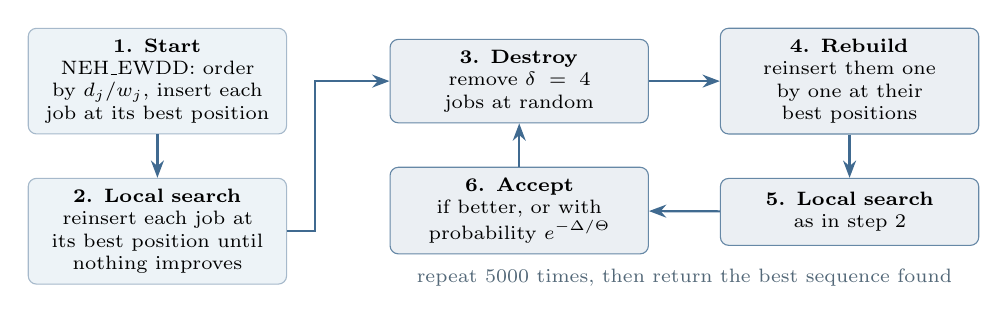
\begin{tikzpicture}[node distance=0.55cm and 0.9cm]
\node[box] (start) {\textbf{1. Start}\\NEH\_EWDD: order by $d_j/w_j$, insert each job at its best position};
\node[box,below=of start] (ls0) {\textbf{2. Local search}\\reinsert each job at its best position until nothing improves};
\node[loopbox,right=1.3cm of start] (destroy) {\textbf{3. Destroy}\\remove $\delta=4$ jobs at random};
\node[loopbox,right=of destroy] (rebuild) {\textbf{4. Rebuild}\\reinsert them one by one at their best positions};
\node[loopbox,below=of rebuild] (ls) {\textbf{5. Local search}\\as in step 2};
\node[loopbox,below=of destroy] (accept) {\textbf{6. Accept}\\if better, or with probability $e^{-\Delta/\Theta}$};
\draw[arr] (start) -- (ls0);
\draw[arr] (ls0.east) -- ++(0.35,0) |- (destroy.west);
\draw[arr] (destroy) -- (rebuild);
\draw[arr] (rebuild) -- (ls);
\draw[arr] (ls) -- (accept);
\draw[arr] (accept) -- (destroy);
\path ($(accept.south)!0.5!(ls.south)$) node[tag,below=0.12cm] {repeat 5000 times, then return the best sequence found};
\end{tikzpicture}
\end{center}
\vspace{-0.1cm}
\small
\begin{columns}[T,onlytextwidth]
\begin{column}{0.5\textwidth}
\begin{itemize}
\item Solution: a permutation of the jobs.
\item Compare: weighted tardiness, then waiting.
\item $\delta=4$, $\lambda=0.5$, $\Theta = \lambda \sum_{j,k} p_{jk} / (10\,n\,m)$ \cite{ruiz2008igwt}.
\end{itemize}
\end{column}
\begin{column}{0.47\textwidth}
\begin{itemize}
\item Stop: 5000 iterations, seed 522; a 300 s cap is only a safety limit.
\item Start from the better of NEH\_EWDD and EDD, so the result is never worse than the rule.
\end{itemize}
\end{column}
\end{columns}
\end{frame}

\section{Experiment design (0:40)}\label{sec:design}
\begin{frame}{Four instances, one checker, 180 paired scenarios}
\begin{columns}[T,onlytextwidth]
\begin{column}{0.5\textwidth}
\begin{block}{Instances and settings}
\footnotesize
\begin{tabular}{lrr}
\toprule
Instance & Jobs & Stages \\
\midrule
Hand-checkable & 6 & 4 \\
Small development & 15 & 8 \\
Medium development & 45 & 8 \\
Large development & 120 & 8 \\
\bottomrule
\end{tabular}
\par\medskip
Iterated greedy: 5000 iterations, seed 522. The independent checker computes every reported value.
\end{block}
\end{column}
\begin{column}{0.47\textwidth}
\begin{block}{Stress test on the 45-job instance}
\footnotesize
\begin{itemize}
\item Each planned time is multiplied by a lognormal factor with mean one and coefficient of variation $\nu$.
\item 30 saved scenarios at $\nu = 0.2$, then 30 new ones at each of $\nu = 0.1$, 0.2, 0.3, 0.5, and 0.8.
\item Both sequences stay fixed; each operation starts as early as the realized times allow.
\end{itemize}
\end{block}
\end{column}
\end{columns}
\end{frame}

\section{Results (3:20)}\label{sec:results}
\begin{frame}{On the hand-checkable case it reaches the optimum: 233 against 281}
\begin{center}
{\scriptsize\color{muted}EDD rule: J001, J002, J005, J003, J006, J004}\\
\gantt{\eddschedule}\\[0.1cm]
{\scriptsize\color{muted}Iterated greedy: J001, J002, J003, J004, J006, J005}\\
\gantt{\igschedule}
\par\smallskip
\weightkey
\end{center}
\point{Explain the gain.}{Moving the weight-1 job J005 last lets the weight-4 jobs finish earlier: J003 at 97 instead of 108 and J004 at 119 instead of 139.}
\point{State the check and the cost.}{All 720 sequences confirm 233 is optimal; waiting rises from 13 to 37 job-minutes.}
\end{frame}

\begin{frame}{On exact data, iterated greedy (IG) is lower than EDD on all four instances}
\begin{center}
\small
\setlength{\tabcolsep}{4pt}
\begin{tabular}{lrrrrrrrrr}
\toprule
 & & \multicolumn{2}{c}{Weighted tardiness} & \multicolumn{2}{c}{Waiting (job-min)} & \multicolumn{2}{c}{Makespan} & \multicolumn{2}{c}{On-time fraction} \\
\cmidrule(lr){3-4}\cmidrule(lr){5-6}\cmidrule(lr){7-8}\cmidrule(lr){9-10}
Instance & Jobs & EDD & IG & EDD & IG & EDD & IG & EDD & IG \\
\midrule
Hand-checkable & 6 & 281 & 233 & 13 & 37 & 139 & 136 & 0.000 & 0.000 \\
Small & 15 & 1,417 & 21 & 732 & 252 & 417 & 357 & 0.333 & 0.867 \\
Medium & 45 & 2,371 & 58 & 2,040 & 794 & 781 & 751 & 0.244 & 0.911 \\
Large & 120 & 23,015 & 4,383 & 7,863 & 3,005 & 1,812 & 1,804 & 0.233 & 0.642 \\
\bottomrule
\end{tabular}
\end{center}
\small
\begin{itemize}
\item All eight decisions pass the checker. Iterated greedy (IG) takes 0.21, 0.52, 3.22, and 37.2 seconds; EDD takes under a millisecond.
\item HiGHS proves 233 and 21 optimal on the 6- and 15-job instances, and iterated greedy reaches both. At 15 jobs the solver's one optimal order has 323 job-minutes of waiting, 71 more than iterated greedy's.
\item At 120 jobs, 5000 iterations have not converged: five other seeds reached 4,159 to 4,306.
\end{itemize}
\end{frame}

\begin{frame}{The gain relative to EDD is largest at 15 and 45 jobs}
\begin{center}
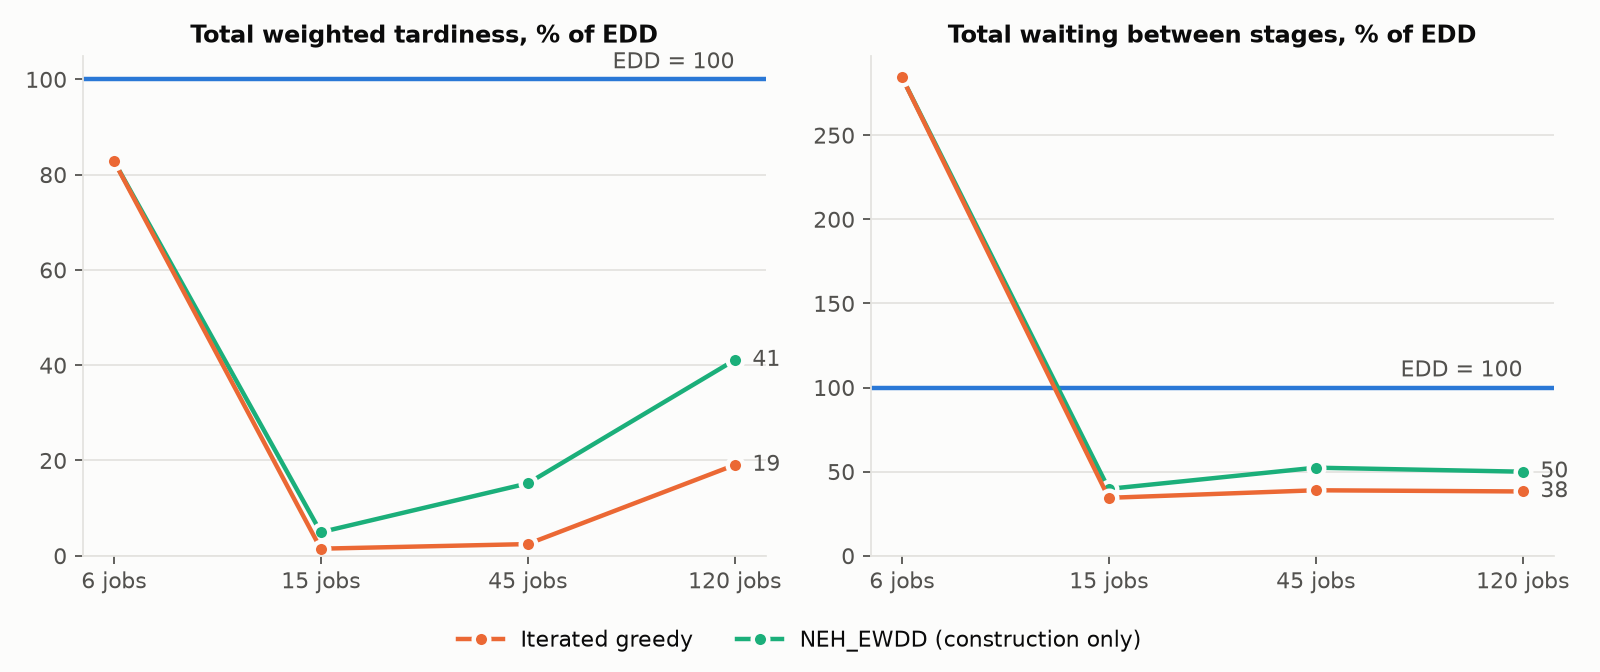
\includegraphics[width=0.86\textwidth]{comparison/comparison.png}
\end{center}
\small
\point{Read the figure.}{At 120 jobs iterated greedy keeps 19 percent of the EDD tardiness; five other seeds there reached 4,159 to 4,306, so the search has not converged.}
\end{frame}

\begin{frame}{At $\nu = 0.2$ the iterated greedy sequence wins all 30 scenarios}
\begin{center}
\footnotesize
\begin{tabular}{lrrrrrr}
\toprule
 & \multicolumn{3}{c}{Weighted tardiness} & \multicolumn{3}{c}{Waiting (job-minutes)} \\
\cmidrule(lr){2-4}\cmidrule(lr){5-7}
Sequence & Planned & Mean & 90th pct. & Planned & Mean & 90th pct. \\
\midrule
Earliest due date & 2,371.0 & 3,541.1 & 4,616.6 & 2,040.0 & 2,454.5 & 2,768.6 \\
Iterated greedy & 58.0 & 420.6 & 592.2 & 794.0 & 1,276.9 & 1,454.9 \\
\bottomrule
\end{tabular}
\par\smallskip
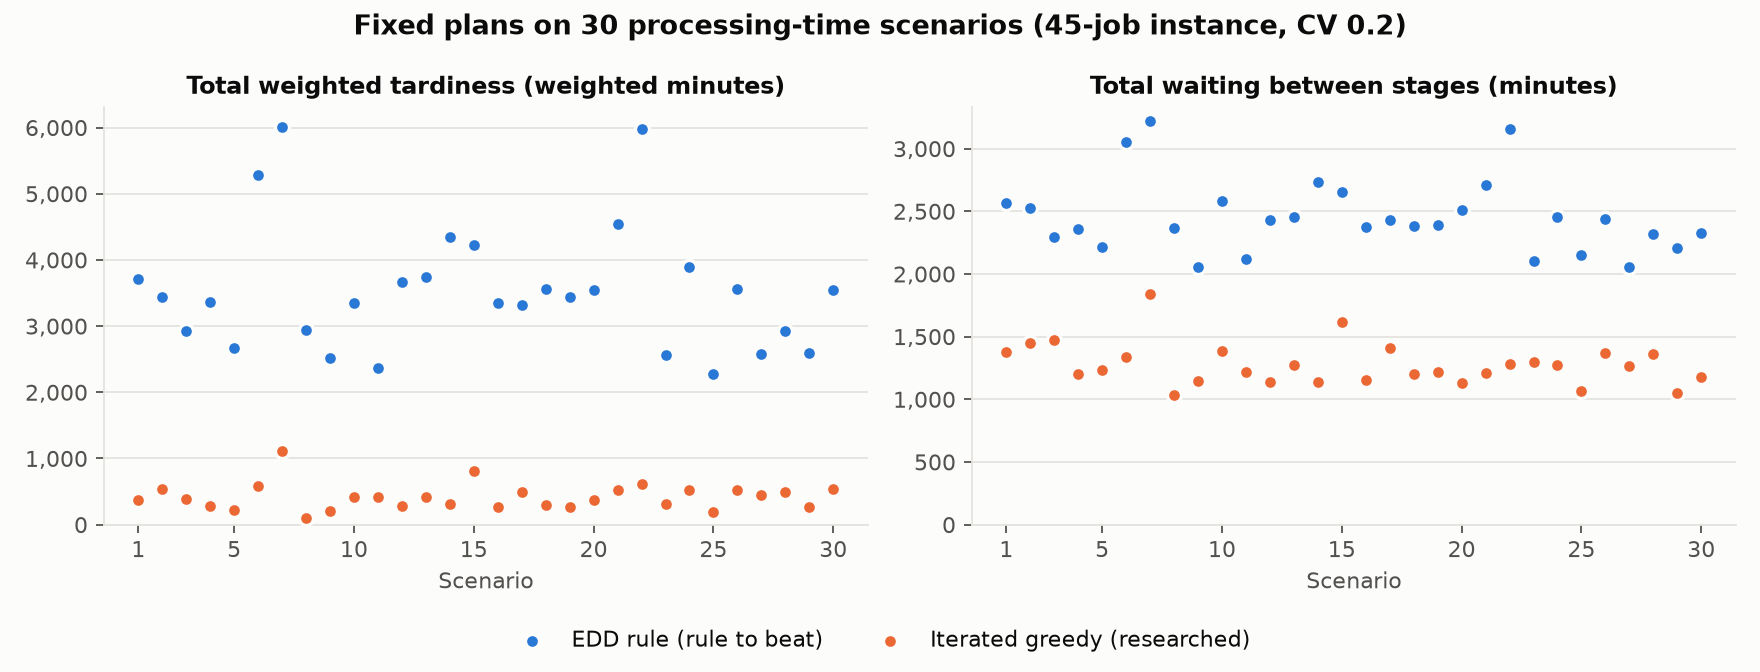
\includegraphics[width=0.74\textwidth]{stress/stress_per_scenario.png}
\end{center}
\vspace{-0.2cm}
{\small\color{uablue}Mean reduction: 3,120.5 weighted minutes (standard error 150.1). No hard constraint is broken.\par}
\end{frame}

\begin{frame}{As variability grows, the percentage falls and the mean gain holds}
\begin{columns}[T,onlytextwidth]
\begin{column}{0.56\textwidth}
\scriptsize
\setlength{\tabcolsep}{3pt}
\begin{tabular}{rrrrrr}
\toprule
 & \multicolumn{2}{c}{Mean tardiness} & \multicolumn{3}{c}{Reduction} \\
\cmidrule(lr){2-3}\cmidrule(lr){4-6}
$\nu$ & EDD & IG & Mean (s.e.) & 10th pct. & \% \\
\midrule
0.1 & 2,720.1 & 148.1 & 2,572.0 (65.9) & 2,048.3 & 94.6 \\
0.2 & 3,273.5 & 407.2 & 2,866.4 (121.3) & 2,055.3 & 87.6 \\
0.3 & 4,139.8 & 952.5 & 3,187.3 (203.8) & 1,781.1 & 77.0 \\
0.5 & 6,680.4 & 2,996.7 & 3,683.7 (223.8) & 2,473.2 & 55.1 \\
0.8 & 12,230.5 & 8,901.6 & 3,329.0 (342.7) & 851.5 & 27.2 \\
\bottomrule
\end{tabular}
\par\medskip
\small
EDD wins 1 of the 180 paired scenarios, at $\nu = 0.8$, by 870.4 weighted minutes.
\end{column}
\begin{column}{0.42\textwidth}
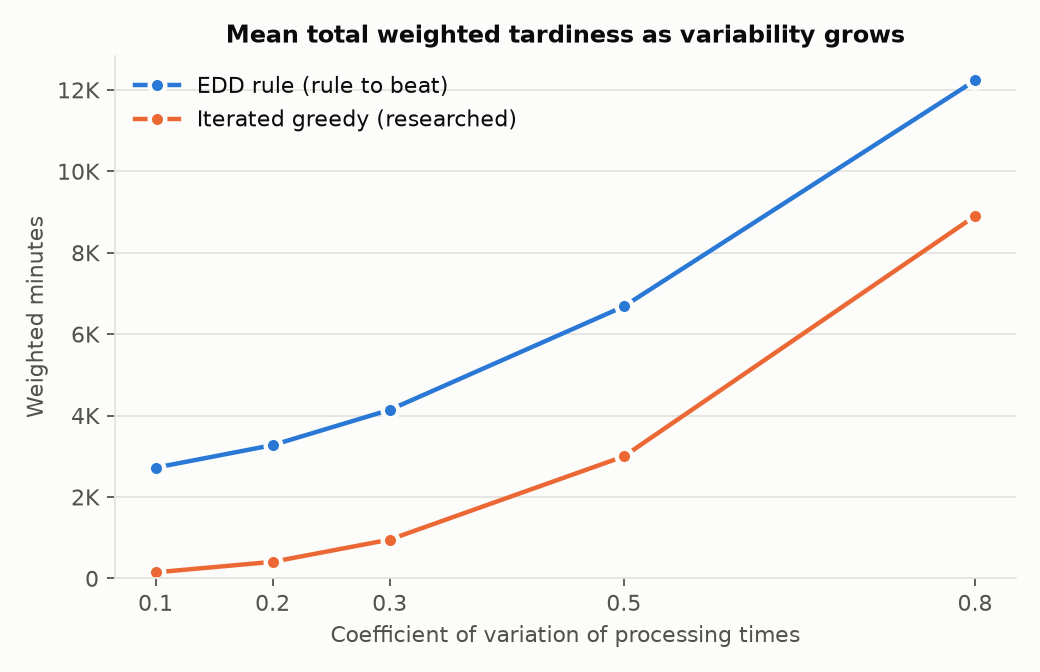
\includegraphics[width=\textwidth]{stress/stress_cv_sweep.png}
\end{column}
\end{columns}
\point{Read the sweep.}{The percentage falls at every step. The mean gain stays between 2,572.0 and 3,683.7 weighted minutes.}
\end{frame}

\begin{frame}{Why: more on-time jobs to lose, each at lower risk}
\begin{center}
\small
\begin{tabular}{lrr}
\toprule
At $\nu = 0.2$, 30 saved scenarios & EDD & Iterated greedy \\
\midrule
Late jobs in the plan & 34 & 4 \\
Mean late jobs across scenarios & 36.1 & 11.5 \\
On-time jobs in the plan & 11 & 41 \\
Median planned slack of on-time jobs (minutes) & 28 & 31 \\
Median simulated completion standard deviation (minutes) & 9.9 & 8.3 \\
Mean late probability of an on-time job & 27.9\% & 18.5\% \\
On-time jobs that turn late per scenario & 3.1 & 7.6 \\
\bottomrule
\end{tabular}
\end{center}
\point{Say what the simulation adds.}{Simulated completion times include the delays passed on by the jobs ahead.}
\end{frame}

\section{Recommendation and limits (0:55)}\label{sec:recommend}
\begin{frame}{Recommendation: use the iterated greedy sequence on this line}
\begin{block}{Expected benefit at $\nu = 0.2$ on the 45-job instance}
\small
Mean weighted tardiness falls by 3,120.5 (standard error 150.1) and, in a second independent set, by 2,866.4 (standard error 121.3). Late jobs per period: 11.5 against 36.1. Mean waiting is 48.0 percent lower.
\end{block}
\begin{block}{Trade-off we accept}
\small
The sequence cannot be traced by hand, depends on a seed, and takes seconds to compute: 3.22 at 45 jobs and 37.2 at 120.
\end{block}
\begin{block}{Condition that would change it}
\small
At $\nu = 0.8$ the mean gain remains 3,329.0, but the 10th percentile of the per-period gain falls to 7.0 percent of the EDD mean and EDD wins 1 of 30 scenarios. Measure the line's variability first.
\end{block}
\end{frame}

\begin{frame}{Limits of the evidence and what comes next}
\begin{columns}[T,onlytextwidth]
\begin{column}{0.53\textwidth}
\begin{block}{What the study does not show}
\footnotesize
\begin{itemize}
\item One generator; the stress test covers one 45-job instance.
\item Independent noise: no slow shift or degraded machine.
\item EDD is a frozen list, not online dispatching.
\item NEH\_EWDD and stochastic methods were not run in the scenarios.
\item Optimality is proven only up to 15 jobs.
\end{itemize}
\end{block}
\end{column}
\begin{column}{0.44\textwidth}
\begin{block}{Next tests}
\footnotesize
\begin{itemize}
\item Score sequences over sampled scenarios.
\item Add correlated delays by stage or shift.
\item Re-sequence at each release.
\end{itemize}
\end{block}
\end{column}
\end{columns}
\end{frame}

\section{Walk-throughs (1:25)}\label{sec:walk}
\begin{frame}{Walk-through (Don): the mixed-integer benchmark}
\framesubtitle{Drafted by Claude Code}
\begin{block}{What it does}
\small Builds the positional program and certifies the optimum of the 6- and 15-job instances with HiGHS.
\end{block}
\begin{block}{What was wrong in the agent's version}
\small It set the objective with a call that also solves, then solved again. The solver reported 81 seconds, but the command took more than three minutes.
\end{block}
\begin{block}{How we checked it}
\small We compared the reported time with the wall clock and removed the second solve. A test requires the proven optimum of 233, and the checker confirms the solver's order.
\end{block}
\end{frame}

\begin{frame}{Walk-through (Amir): which on-time jobs are at risk}
\framesubtitle{Drafted by Claude Code}
\begin{block}{What it does}
\small Measures how exposed the on-time jobs of each sequence are when processing times vary.
\end{block}
\begin{block}{What was wrong in the agent's version}
\small It compared slack with the variation of a job's own processing times. That misses delays passed on by the jobs ahead.
\end{block}
\begin{block}{How we checked it}
\small We replaced it with simulated completion times over the 30 saved scenarios. Jobs with slack below that variation became 6 of 41 and 4 of 11, where the first version showed 3 in each sequence.
\end{block}
\end{frame}

\begin{frame}{What we now know}
\small
\begin{itemize}
\item On exact data, iterated greedy cuts weighted tardiness by 81.0 to 98.5 percent against EDD on the development instances and reaches the proven optimum on the two smallest instances.
\item At $\nu = 0.2$, its fixed sequence wins all 30 scenarios, with an 88.1 percent lower mean.
\item As variability grows, the percentage falls to 27.2 at $\nu = 0.8$, while the mean gain stays between 2,572.0 and 3,683.7 weighted minutes.
\end{itemize}
\point{State the message.}{A plan optimized on wrong times kept its value on this line at every level of variability we tested.}
\end{frame}

\section{Sources}\label{sec:sources}
\begin{frame}[allowframebreaks]{Sources}
\scriptsize
\bibliographystyle{unsrturl}
\bibliography{Option6_Prototype_Slides}
\end{frame}
\end{document}
